% this file is called up by thesis.tex
% content in this file will be fed into the main document

%------------------------------------------------------------------------- 

\chapter{Caracterización de aberraciones en Vórtices Ópticos}
\label{cha:Car_intro}
\graphicspath{{Figures/chPD_img/}{../Figures/chPD_img/}}
\lhead{Caracterización de aberraciones en Vórtices Ópticos:
  \textit{Introducción}} % This is for the header on each page -
                         % perhaps a shortened title
\section{Introducción}
En capítulos anteriores ha quedado claro que para producir VO es
necesario contar con un sistema óptico en el cual sea posible
manipular con precisión la fase de un frente de onda.  Asimismo, se
presentó un montaje experimental en el cual logramos generar VO a
partir del uso de dispositivos difractivos conocidos como SLMs. 
No obstante, los VO obtenidos distan de ser de suficiente calidad como
para ser usados en aplicaciones científicas o tecnológicas. 

Esta segunda parte de la tesis abarca el trabajo que se realizó para
mejorar la calidad óptica de nuestro montaje con el fín de mejorar los
VO que se obtuvieron en la parte anterior. 

\section{Estado del Arte}
\label{sec:ChPD_estado_del_arte}
\lhead{Caracterización de aberraciones en Vórtices Ópticos: \textit{Estado
    del Arte}}

Los sistemas ópticos formadores de imágen que se encuentran en
aplicaciones de la vida real están sujetos a aberraciones de fase que
limitan su resolución. Es por ello que en la industria y en laboratorios se hace un gran esfuerzo para
detectar aberraciones y corregirlas vía Óptica Adaptativa (AO) \citepChPD{Kubby2013} o por
medio de técnicas digitales posteriores a la adquisición
\citepChPD{Korkiakoski2012}. 

Las aberraciones ópticas en un sistema formador de imagen pueden
proceder de fuentes intrínsecas tales como imperfecciones en el
diseño, los materiales, la manufactura o la alineación de los
elementos que los componen. O de fuentes extrínsecas como variaciones
en el índice de refracción de muestras microscópicas y turbulencia atmosférica en
imágenes capturadas usando telescopios. La presencia de aberraciones
del último tipo en imágenes procedentes de telescopios terrestres, y
la dificultad de modificar los sistemas para incluir brazos de referencia han sido la motivación para
el desarrollo de varias técnicas de Sensado de Fase no
Interferométricas (NI-WFS). La técnica de Diversidad de Fases o Phase
Diversity (PD) pertenece a una familia de NI-WFS conocida como de
Reconstrucción de Fase o Phase Retrieval. A diferencia de técnicas
directas que requieren de óptica y sensores adicionales como los
sistemas que usan sensores Shack-Hartman, las técnicas de Phase
Retrieval consisten en la determinación de la fase de una función
compleja a partir de medidas de su magnitud usando 
información a priori de la función o de su transformada \citepChPD{Fienup1993}. 
Específicamente, la técnica de reconstrucción  PD ha sido usada
exitosamente en el contexto de sistemas de AO para incrementar la resolución de sistemas ópticos
tales como el Telescopio Espacial Hubble \citepChPD{Fienup1993}, y en
post procesamiento de imágenes de astronomía en las cuales la
resolución es crítica. Dos casos muy relevantes son el estudio de
manchas solares y la detección de planetas extrasolares \citepChPD{Lofdahl1994,Bonet2005,Korkiakoski2012,Sauvage2007,Sauvage2012}. 

Así como con otras técnicas desarrolladas para aplicaciones en
astronomía, los métodos de reconstrucción de fase como el
Gerchberg-Sachston (GS) y PD han migrado a aplicaciones en el
laboratorio, y más específicamente a aplicaciones en microscopía de
fase \citepChPD{Jesacher2007,Camacho2010,Kner2013a}. Tal es el caso
del trabajo de \citetChPD{Jesacher2007} que implementó una versión del
método GS para la optimización de pinzas ópticas utilizadas como
iluminación en sistemas de microscopía de contraste de fase espiral. 

En este capítulo se presenta un método novedoso de reconstrucción de
fase del tipo PD inspirado en la aplicación antes mencionada, y por
medio del cual fue posible detectar y corregir las aberraciones ópticas
del sistema generador de VO presentado en el capítulo
\ref{cha:Gen_intro}.  A continuación, se presenta el marco teórico que
soporta la implementación del método. En la sección
\ref{sec:ChPD_materiales_y_metodos} se presenta el montaje óptico y se
describe el algorítmo general para la reconstrucción de fase. Lugo, en
la sección \ref{sec:ChPD_resultados} se presentan los resultados de
simulaciones y experimentos que permiten corroborar la efectividad del
método para la corrección de aberraciones. 

\section{Marco Teórico}
\label{sec:ChPD_marco_teorico}
Los métodos de reconstrucción de fase no interferométricos dependen de
la medida de la intensidad de la intensidad del campo óptico que se
propaga a traves de un sistema formador de imagen. Si el sistema
formador de imagen se
caracteriza por su Función de Dispersión de Punto (PSF), la intenidad
a la salida puede ser descrita como una convolución entre la imagen a
la entrada y la PSF tal y como se ilustra en la ecuación
(\ref{eq:Output_Image}).
\begin{equation}\label{eq:Output_Image}
d(\vec{x}) = d_{obj}(\vec{x}) \otimes s(\vec{x}).
\end{equation}
En este caso hemos usado la notación de \citetChPD{Paxman1992} dónde
la PSF se representa como $s$, $d_{obj}$ es la intensidad del objeto a
la entrada y $d$ es la intensidad de la imagen a la salida, todas
ellas evaluadas en el espacio de coordenadas naturales ($\vec{x}$). El
 \href{http://es.wikipedia.org/wiki/Teorema_de_convolución}{Teorema de
   Convolución} permite representar la operación de la expresión
 (\ref{eq:Output_Image}) como un simple producto punto entre las
 Transformadas de Fourier (FT) de la intensidad a la entrada y la
 PSF como se muestra a continuación. 
\begin{equation}\label{eq:Output_Image_fourier}
D(\vec{u}) = D_{obj}(\vec{u})S(\vec{u}).
\end{equation}
En \ref{eq:Output_Image_fourier} el término $S$ denota la Función de
Transferencia Óptica (OTF) del sistema formador de imagen, y así como
con los otros términos, letras mayúscula denotan una transformada de
Fourier sobre la función con notación minúscula.
\begin{align*} 
S(\vec{u})&= \mathcal{F}\{ s(\vec{x}) \},&D(\vec{u})&= \mathcal{F}\{ d(\vec{x}) \}, &D_{obj}(\vec{u})&= \mathcal{F}\{ d_{obj}(\vec{x}) \}. 
\end{align*}
Hasta el momento hemos trabajado únicamente con funciones reales que
representan la intensidad del campo punto a punto en los planos objeto
e imagen de un sistema óptico. Este tipo de notación es de grán utilidad para las
aplicaciones clásicas del método PD que hacen imágen de objetos
lejanos, y con fuentes de iluminación no coherentes. Sin embargo, en
sistemas ópticos con fuentes de iluminación coherentes, como el que se presentó en la primera parte de este documento
para la generación de VO, tenemos la ventaja de trabajar con
campos complejos que proporcionan información de amplitud y fase. Para
adaptar el método clásico de PD a una versión de iluminación coherente
es necesario trabajar con campos complejos. Es bien sabido que la OTF
y la PSF forman un par de Fourier en el dominio no coherente, y cada
una de ellas tiene un equivalente en el dominio de la luz
coherente. Por una parte, la contraparte coherente de la PSF es la
Función de Respuesta al Impulso en amplitud o PSF de amplitud y de
aquí en adelante se denotará como $h(\vec{x})$. La PSF es el módulo
cuadrado de la PSF de amplitud (APSF), 
\begin{equation}\label{eq:PSF}
s(\vec{x}) = |h(\vec{x})|^2.
\end{equation}
Y así
como la PSF relaciona intensidades de campo a la entrada y salida de
un sistema por medio de una convolución, la PSF de amplitud relaciona
los campos ópticos complejos.
 \begin{equation}\label{eq:Output_Image_complex}
u(\vec{x}) = u_{obj}(\vec{x}) \otimes h(\vec{x}).
\end{equation}
Del otro lado, el equivalente coherente de la OTF es la Función de
Transferencia Óptica de amplitud, o Pupila Generalizada del sistema
(GP) y por ser el par de Fourier de la APSF se cumple la relación (\ref{eq:GP}). 
\begin{equation}\label{eq:GP}
 H(\vec{u}) = \mathcal{F} \{h(\vec{x})\} =  A(\vec{u}) e^{i\phi(\vec{u})}
\end{equation}
En (\ref{eq:GP}) se observa que fuera de ser la FT de la APSF, la GP es
una función compleja que describe tanto la forma y
tramitancia de la apertura $A(\vec{u})$ como la fase del sistema
óptico $\phi(\vec{u})$. \\
La OTF de un sistema formador de imágen con iluminación coherente se
puede obtener mediante la autocorrelación normalizada de la GP como se
muestra a continuación.
\begin{equation}\label{eq:OTF}
S(\vec{u}) = \frac{H(\vec{u}) \star H(\vec{u})}{|H(\vec{u})|^2}
\end{equation}

Todo lo mencionado anteriormente ha sido ingeniosamente condensado por
\citetChPD{UribePatarroyo2011} en una versión de la figura
\ref{fig:ChPD_kernels_sistemas_formadores_de_imagen}. 
\begin{figure}[h!]
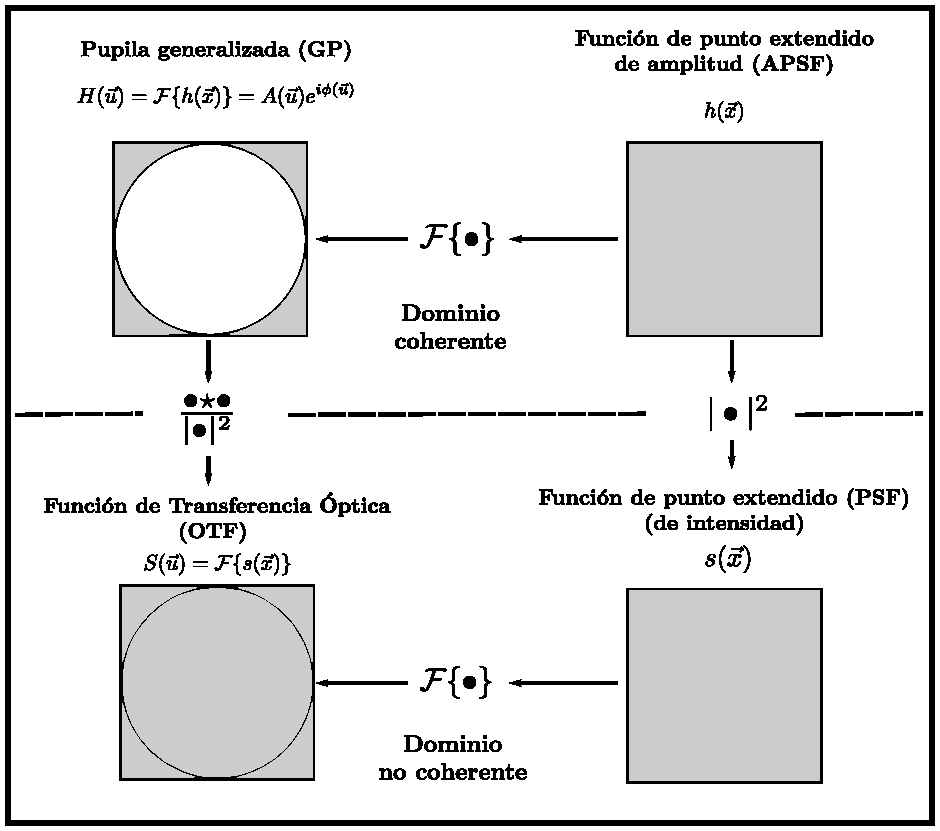
\includegraphics[scale=1]{kernels_sistemas_formadores_de_imagen.pdf}
\caption[Relaciones entre funciones de transferencia ópticas y sus FT.]{Relaciones entre funciones de transferencia ópticas y sus
  transformadas de fourier en los dominios coherente y no
  coherente. Inspirado en una versión similar de \citetChPD{UribePatarroyo2011}.}
\label{fig:ChPD_kernels_sistemas_formadores_de_imagen}
\end{figure} 

Ahora bien, las expresiones (\ref{eq:PSF}) y (\ref{eq:OTF}) nos
permiten llevar sistemas ópticos descritos por campos complejos a la
notación tradicional del PD. A continuación se describen los aspectos
 generales de la reconstrucción de fase con PD, y en la sección
 \ref{sec:ChPD_PD_il_coherente} se describirán las modificaciones que
 hacemos al PD tradicional para aprovechar el tipo de iluminación no
 coherente.

\subsection{PD tradicional}
\label{sec:ChPD_PD_tradicional}
Si la GP del sistema es modificada por cambio conocido en la fase de
la forma:
$$H_{\Delta}=e^{\phi_1(\vec{u})}$$ 

\subsection{PD con iluminación coherente}
\label{sec:ChPD_PD_il_coherente}

\section{Materiales y Métodos}
\label{sec:ChPD_materiales_y_metodos}

\section{Resultados}
\label{sec:ChPD_resultados}

\newpage
\pagebreak[4]
\bibliographystyleChPD{unsrtnat}
\bibliographyChPD{References/Ch_PD}